The concept of dataspaces was the first time presented in 2005 and describes a new abstraction of data management \cite[p. 27]{Franklin:2005:DDN:1107499.1107502}. 
The motivation for a new type of data management arises from the issue that rarely the data to be managed is solely stored in a convenient relational database, nor is stored in a single data model.
For a long time relational databases were the dominating choice for storing data, but this is changing, as the coming popularity of NoSQL databases indicates \cite{SQL_NOSQL_DATABASES}. Also for multimedia content, relational databases aren't always an ideal choice since they were conceptualized for structured data, whereas multimedia data can contain all types of data. Also distribution is a problem, that is difficult to handle with relational databases, since they were also designed for monolithic use-cases.
We can record that applications have to handle more and more different types of data sources and thus have to handle heterogeneous and distributed data, too.

That issue is ubiquitous and arises in enterprises, government agencies and even on everybody's PC desktop. As example par excellence serves the healthcare sector dealing with highly heterogeneous and complex data, and struggling with a continuously growing amount of data.

%As a result, developers face the challenge to deal with heterogeneous data on a low level base. Challenges are to provide search and query capabilities, enforcing rules, integrity constraints, naming conventions etc.; tracking lineage; providing availability, recovery and access control; and managing evolution of data and meta-data. That issues are ubiquitous and arise in enterprises, government agencies and even on one's PC desktop. 
As a response to this problem, the authors of \cite{Franklin:2005:DDN:1107499.1107502} postulate the concept of dataspaces and corresponding to this the  development of DataSpace Support Platforms (DSSPs). Shortly said, the latter provides an environment of cooperating Services and guaranties that enables software developers to concentrate on their specific application problem rather than taking care of returning issues in consistency and efficiency of huge, linked but heterogeneous data sets. The remarkable properties of a dataspace system are defined as follows \cite[p. 28]{Franklin:2005:DDN:1107499.1107502}:

\begin{itemize}
\item A DSSP must deal with data and applications in a variety of file formats that are accessible through many systems with different interfaces. A DSSP has to support all kinds of data in the dataspace and isn't allowed to omit any ( e.g. as DBMSs do).

\item An integrated possibility for searching, querying, updating and administration is provided by the DSSP, but the data often is also accessible and modifiable through native interfaces. Therefore DSSPs haven't full control over their data.

\item The DSSP can offer several query services, but isn't forced to return the most accurate result. Indeed,  the answers can be approximated resp. \emph{best-effort}. If some data sources e.g. are unavailable for some reason, the dataspace might use the current available data sources and creates the best possible result.

\item Whenever it is required, the DSSP has to provide tools to do tighter data integration.
\end{itemize}

Current data integration systems are essentially a natural extension of traditional databases, where queries are specified in a structured form and data is modeled in one of the traditional data models like relational or XML. The System for data integration also has exact information about how the data in the sources map to the schema used for integration. So, for data integration there is a need for large upfront effort in creating the mediated schema and the schema mappings.

Many of the services a dataspace provide, data integration and exchange systems provide, too. The main difference between these systems is that data integration systems need a semantic integration process before they can provide any services on the data. Additionally, data integration systems always have a global schema. But a dataspace is not a kind of a classic data integration approach. Initially, a dataspace doesn't semantically integrate the data. It allows data to \emph{coexist}.  The idea is to provide base functionality over all data sources, regardless of their specific integration constraints. E.g. a DSSP is able to provide a keyword search similar to a desktop file search. If more sophisticated operations are required, such as relational queries, data mining or monitoring of specific data sources, additional effort can be done to integrate the sources tighter. This incremental process is also called as \emph{pay-as-you-go} data integration.

%Dataspace Support Platforms (DSSP) shall considerable reduce this upfront effort. The system should be able to bootstrap itself and provide useful services with no human intervention. When the data management needs become clearer (through user feedback or as sources are added), the system evolves in a pay-as-you-go fashion.

%\textcolor{red}{\textbf{Stuff that has to be reorganized:}}\\
%\textcolor{red}{Following paragraph have to be moved to more suitable place!}\\
%The document ``Principles of Dataspace System'' of Alon Haley, Michael Franklin and David Meier\cite{Halevy:2006:PDS:1142351.1142352} is based on their previous work ``From Databases to Dataspaces - A New Abstraction for Information Management''\cite{Franklin:2005:DDN:1107499.1107502} where the concept of dataspaces was firstly presented, and poses specific technical challenges realizing Dataspace Support Platforms (DSSPs) relating to query answering, introspection and the benefits of human attention for improving semantic relationships within a dataspace.  
%In the following are stated the results of the above mentioned challenges:


%In the paper ``Towards Realization of Dataspaces'', written by Ibrahim Elsayed and Peter Brezany\cite{1698348}, the architecture and functionality of a Dataspace Management System(DMS) is presented. Additionally it is discussed, how grid technology of future implementations is able to support such an architecture. A DMS is a set of software programs, which controls the organization, storage and retrieval of data in a Dataspace. It also handles the security and integrity of a Dataspace.
%In the following, the architecture and the functionality requirements of a DMS will be described.   

A Dataspace should contain all information being relevant for a specific organization/task, regardless of their file format or storage location, and it should model a collection of relationships between the data sources. Therefore the dataspace is defined as a set of participants and relationships \cite[p. 29]{Franklin:2005:DDN:1107499.1107502}. 
Participants of a dataspace are individual data sources. 
Some participants support expressive query languages for querying, while others only provide limited access interfaces. 
Participants can reach from structured, semi-structured right up to unstructured data sources. Some sources provide traditional updates, some are only be appendable, while others are immutable. Further, dataspaces can be nested within each other, which means that a dataspace should be able to be a part of another dataspace.  Thus, a dataspace has to provide methods and rules for accessing its sub dataspaces.

Not every participant will provide all necessary interfaces for being able to support all DSSP features \cite[p. 29]{Franklin:2005:DDN:1107499.1107502}. 
Hence, it is necessary that data sources can be extended on various ways. E.g. a source don't store its own meta-data, so there has to be an external meta-data repository for it. 

A DSSP should also support updating data \cite[p. 29]{Franklin:2005:DDN:1107499.1107502}. Of course, the mutability of the relevant data sources determines the effects of updates.  
Other key services would be monitoring, event detection and the support for complex workflows (e.g. is desired that a calculation is done if new data arrives and that the result will be distributed over a set of data sources) \cite[p. 29]{Franklin:2005:DDN:1107499.1107502}. On a similar way a DSSP should support various forms of data mining and analysis. 
The user should be able to discover relevant datasources and to look for their completeness, correctness and recency \cite[p. 29]{Franklin:2005:DDN:1107499.1107502}. A DSSP indeed should recognise when data of the domain is incomplete. 

\section{Components and Services}

In this section we will look at the components forming a fully-fledged dataspace and the services providing these components. Figure \ref{TowardsRealizationOfDataspacesEnvironment} shows the components as they were defined in \cite{1698348}:


\begin{figure}[H]
	\begin{center}
		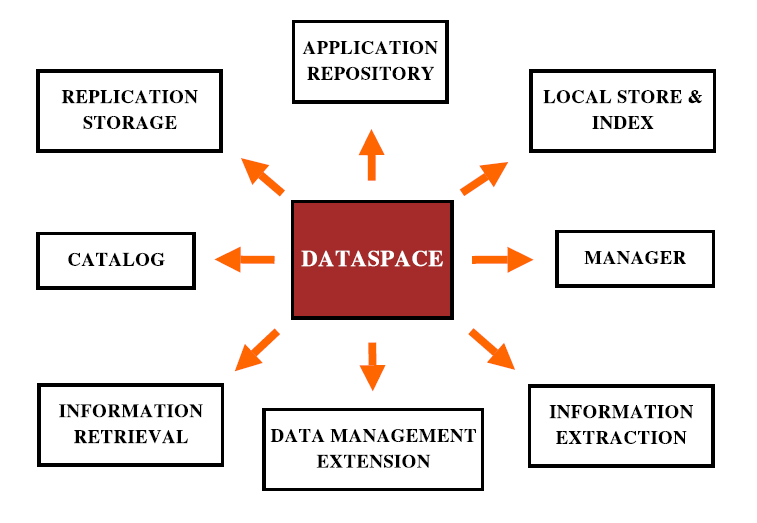
\includegraphics[width=0.75\textwidth]{figures/TowardsRealizationOfDataspaces1.png}
	\end{center}
	\caption{Environment of  a Dataspace \cite[p. 2]{1698348}}
	\label{TowardsRealizationOfDataspacesEnvironment}
\end{figure}

\uline{\textbf{Catalog:}} 
The most basic service a dataspace should provide is the cataloging of data elements of all participants. A catalog is an inventory of data resources containing all important information about every element (source, name, storage location inside the source, size, creation date, owner, etc.) of the dataspace. 
It is important that the catalog includes the schema of the source, statistics, rates of change, accuracy, completeness query answering capabilities, ownership, and access and privacy policies for each participant. 
Relationships may be stored as query transformations, dependency graphs, or even textual descriptions.The catalog is the infrastructure for the most other dataspace services. Search and query are two main services a DSSP must provide. A user should be able to state a search query and iteratively precise it, when appropriate, to a database-style query. For the dataspace approach it is a key tenet that search should be applicable to all of the contents, regardless of their formats.
The search should include both, data and meta-data. Then, it can support basic browsing over the participant's inventories. The catalog may reference a meta-data repository to separate the basic and more detailed descriptions.
It isn't a very scalable interface, but it can be used to response to questions about the presence or absence of a data element, or determine which participants have documents of a specific type. 
On top of the catalog the DSSP should have a model-management environment allowing the creation of new relationships and manipulation of existing ones.

\uline{\textbf{Information Retrieval:}} The Information Retrieval component (in \cite{Halevy:2006:PDS:1142351.1142352} stated as 'Search and Query') can be split up into queries and searches, two different methods of information retrieval, and represent together one of the main services a DSSP should support. 
Generally, queries and searches should be supported by all participants of the Dataspace, regardless of their used data model. 
It shouldn't make any difference for a user to operate on a sole database or on a Dataspace. 
A good known and simple search operation is keyword searching. 
The support of spanning such a search method over all participants is a challenging research topic: The development of methods for keyword searching on relational and XML databases was done by the data-engineering community \cite{994693, Guo:2003:XRK:872757.872762, Hristidis:2002:DKS:1287369.1287427}. 
For to support a global query functionality allowing to formulate uniform queries on all Dataspace participants, intelligent methods for interpreting and translating of queries in several languages are required. Methods for query translation were investigated by a large body of research communities \cite{Carey00xperanto:publishing, 1319983}.
In the following are listed the main requirements having to be supported by this component:

\begin{description}
\item [Query everything:]  any data item should be queryable  by the user regardless of the file format or data model. 
Keyword queries initially should be supported. 
When more information about a participant is collected, it should be possible to gradually support more sophisticated queries. 
The transition between keyword query, browsing and structured querying should be gracefully. 
Also, when answers are given to keyword (or structured) queries, the user should be able to refine the query through additional query interfaces. 

\item [Structured queries:] queries similar to database ones should be supported on common interfaces (i.e. mediated schemas) that provide access to multiple sources, or can be posed on a specific data source (using its own schema). The intention is, that answers will be obtained also from other sources (as in peer-data management systems). Queries can be posed in a variety of languages (and underlying data models), and should be translated into other data models and schemas as best as possible with the use of exact and approximate semantic mappings.

\item [Meta-data queries:] it is of essential importance that the system supports a huge variety of meta-data queries. These include (a) source inclusion of an answer or how it was derived or computed, (b) time steps provision of the data items that are included in the computation of an answer, (c) specification of whether other data items may depend on on a particular data item and the ability to support hypothetical queries. A hypothetical question would be 'What would change if I removed data item X?' (d) Querying the sources and degree of uncertainty about the answers.
Queries locating data, where the answers are data sources rather than specific data items, should be supported, too. 

\item [Monitoring:] all stated Search and Query services should also be supported in an incremental form which is also applicable in real-time to streaming or modified data sources. It can be done either as a stateless process, in which data items are considered individually, or as a statefull process. In the latter multiple data items are considered.   
\end{description}

\uline{\textbf{Local Store and Index:}} This component is responsible for caching search and query results, so that certain queries can be answered without the need of accessing the actual data sources. Furthermore it supports the creation of queryable associations between the participants. The component should try to achieve the following goals:
\begin{itemize}
\item to create efficiently queryable associations between data items in different participants. Important is here, that the index should identify information across participants when certain tokens appear in multiple ones (in a sense, a generalization of a join index)

\item to improve accesses to data items with limited access patterns. Here, the index has to be robust in the face of multiple references to real-world objects, e.g. different ways to refer to a company or person.

\item to answer certain queries without accessing actual data sources. Thus, the query load is reduced on participants which cannot allow ad-hoc external queries. 
  
\item to support high availability and recovery   
\end{itemize}

The index has to be highly adaptive to heterogeneous environments. It should take as input any token appearing in the dataspace and return the location at which the token appears and the roles at each occurrence. Occurrences could be a string in a text file, element in file path, a value in a database, element in a schema, or tag in a XML file. 

\uline{\textbf{Discovery Component:}} This component (not listed in Figure \ref{TowardsRealizationOfDataspacesEnvironment}) locates participants in a dataspace, creates relationships between them, and helps administrators to refine and tighten these relationships. For each participant the component should perform an initial classification according to the participant's type and content. The system should provide an environment for semi-automatically creating relationships between existing participants and refining and maintaining existing ones. This involves both, finding which pairs of participants are likely to be related, and then proposing relationships which a human can verify and refine. The discovery component should also monitor the content in order to propose additional relationships in the dataspace over time.  

\uline{\textbf{Data Management Extensions:}} This component (in \cite{Halevy:2006:PDS:1142351.1142352} stated as \textit{Source Extension Component}) provides possibilities to improve low-level working Dataspace components. All these base components have only limited data management capabilities. It is a task of a DSSP to provide additional functionality such as backup, recovery and replication. Some participants may not provide significant data management functions. For example, a participant might be no more than departmental document repository, perhaps with no services than weekly backups. A DSSP should support to enrich such a participant with additional capabilities, such as a schema, a catalog, keyword search and update monitoring. It may be necessary to provide these extensions locally, as there might exist applications or workflows that assume the current formats or directory structures.	
This component also supports ``value-added'' - information held by the DSSP, but not present in the initial participants. Such information can include ``lexical crosswalks'' between vocabularies, translation tables for coded values, classifications and ratings of documents, and annotations or linked attached data set or document contents. Such information must be able to span participants in order to link related data items.\\

\uline{\textbf{Information Extraction:}} The world-wide web has become a large data container by now. For allowing to postprocess data obtained from the web, techniques for web information extraction, extracting relevant information from semi-structured web pages should be supported. For further processing extracted content has to be converted to structured data, and saved locally. Non structured web documents have first to be classified using text mining techniques, which organize the parsed documents into groups with the help of ontologies \cite{conf/wise/HeQZW04}. Based on these ontologies a keyword search is able to find individual documents. Structured documents allow easier access and integration due to the rich semantically information included in the data representation.\\

\uline{\textbf{Manager:}} In order to realize the above mentioned functionality, a central component managing the system and interacting with the user is needed. Alongside user authentication, right assignments and other services, this manager component is responsible for communicating with all participants. Thus, this component serves as an interface between the users and the participants of the Dataspace.\\

\uline{\textbf{Replication Storage:}} Allows to copy participant data in order to increase its access time. This results in high availability, and high recovery is supported.\\

\uline{\textbf{Application Repository:}} With this component the user is able to share data analysis tools, domain specific models, evaluations, etc., which can be applied to the (available) data of the Dataspace.\\


\section{Query answering}

In a dataspace, queries might be posed in a wide range of different languages \cite[p. 3]{Halevy:2006:PDS:1142351.1142352}. But most of the activities will properly begin with a keyword search, but it might also be common to see queries as a result of a form (which results to queries with several selectable predicates). More complex queries arise when a user interacts deeper with a certain data source. 
If it isn't explicitly stated, it can be assumed that a user likely believes a query considers all relevant data in a dataspace, regardless of the used data model or schema. Even if a query is posed to a data source, it is implicitly expected that the system considers the data of other sources, as well. If additional answers are desired, one has to do transformations on the schema and the data model.

\textbf{Challenges of answer querying}

Answers corresponded to queries of a dataspace are different from traditional queries in several ways. In the following we list challenges a dataspace has to deal with \cite[p. 3-4]{Halevy:2006:PDS:1142351.1142352}:

\begin{itemize}
\item \textbf{Ranking}: Queries are typically sorted by their relevance, similar to a web search engine. Ranking is necessary not only for keyword search, but also for structured queries, when transitions to other data sources should be approximated.  

\item \textbf{Heterogenity}: Answers will come from many sources and will differ in their used data model and schema. The Ranking has to manage heterogeneity, too.

\item \textbf{Sources as answers}: In addition to base elements (e.g. documents or tuples), a DSSP should also be able to provide sources. This means that it returns links to locations where additional answers can be found.

\item \textbf{Iterative queries}: Normally, the interaction with a dataspace can't be reduced to the process of posing  a sole query and getting an answer to it. Instead, a user is involved in an information finding task that requires a sequence of queries, each being a refinement or modification on the previous ones.

\item \textbf{Reflection}: It is expected, that a DSSP reflects on the completeness of its coverage and the accuracy of its answers. 
\end{itemize}


\section{Uncertainty in Dataspaces}
 
In the paper ``Data Modeling in Dataspace Support Systems'' \cite{DBLP:conf/birthday/SarmaDH09}, the authors face the issue of uncertainty in dataspaces. In their view, a dataspace needs to model uncertainty in its core. In their work, they described the concepts of probabilistic mediated schemas and probabilistic mappings as enabling concepts for DSSPs. With this foundation, it is possible to completely bootstrap a pay-as-you-go integration system. 
In order to develop DSSPs, it is impossible to rely on the same data modeling paradigms data integration systems use. 
One cannot assume that the mediated schema is given in advance, and that the schema mappings between the sources and the mediated schema will be accurate. Therefore the authors argue that uncertainty has to be considered in the mediated schema and in the schema mappings.

Now, we discuss the different kinds of uncertainty, that can arise in a dataspace \cite[p. 123]{DBLP:conf/birthday/SarmaDH09}:

\begin{itemize}
\item \textbf{Uncertain mediated schema}: 
the set of schema terms in which queries are posed is called the mediated schema. 
Not necessarily the set covers all the attributes in any source, it  rather covers the aspects of the domain that the developer of the application wishes to expose to the user.
For several reasons uncertainty happens in the mediated schema. First, if the mediated schema is derived from the data sources during bootstrapping, there will be some uncertainty about the results. When domains are broad, there will be also some uncertainty about how to model them, because in general there will be overlappings in different topics. 

\item \textbf{Uncertain schema mapping}: schema mapping defines the semantic relationships between the terms in the sources, and the terms used in the mediated schema. Although, schema mappings can be inaccurate. 
In a dataspace many of the initial schema mappings are probably automatically derived, and therefore they might be inaccurate. 
In general, it is impossible to create and maintain precise mappings between data sources. 

\item \textbf{Uncertain data}: some of the data may be obtained by automatism, as data sources may not always be structured well. Additionally, unreliable or inconsistent data may be contained in systems with many sources.

\item \textbf{Uncertain queries}: probably much of the early interaction with a dataspace will be done through keyword queries, as the users aren't aware of a (non-existent) schema. The queries have to be translated into some structured form so they can be reformulated with respect to the data sources. At this point multiple candidate structured queries could be generated, and thus some uncertainty arises about which query captures the real intention of the user.
\end{itemize} 

The most fundamental characteristic of a dataspace system handling uncertainty is that it is based on a probabilistic data model. In contrast to a traditional data integration system which includes a single mediated schema and assumes a single (and correct) schema mapping between the mediated schema, and each source, the data integration module of a DSSP attaches possibilities to multiple tuples, mediated schemas, schema mappings, and possible interpretations of  keyword queries posed to the system. 

For a database it is assumed that queries are posed as keywords. This is contrary to traditional integration systems which assume the query to be posed in a structured fashion( i.e. that it can be translated to some subset of SQL). So, a DSSP must first reformulate a keyword query into a set of candidate structured queries before it can reformulate the query onto the schemas of the data sources. This step is also called keyword reformulation. 
It is important to note that keyword reformulation differs from keyword search techniques on structured data (see \cite{994693}, \cite{Hristidis:2002:DKS:1287369.1287427}) in that (a) it does not assume access to all data in the sources, or that the sources support keyword search, and (b) tries to distinguish different structural elements in the query in order to pose more precise queries to the sources. In any case keyword reformulation should benefit from techniques that support answering search on structured data.

\begin{figure}[H]
	\begin{center}
		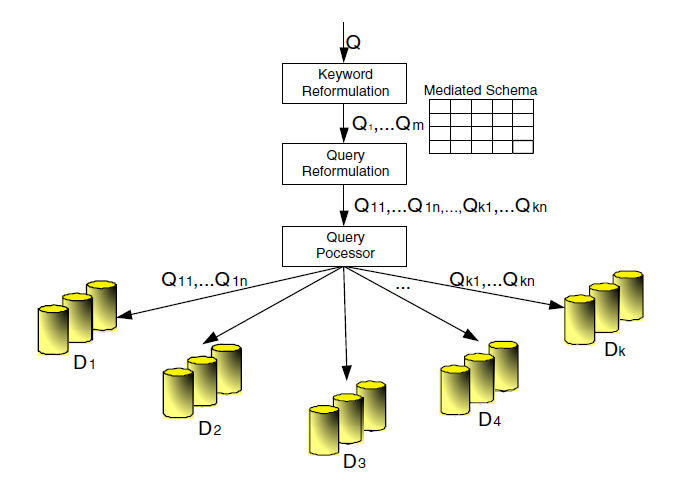
\includegraphics[width=0.75\textwidth]{figures/DataModelingInDSSPs-Figure1.png}
	\end{center}
	\caption{Architecture of a dataspace system that handles uncertainty \cite[p. 124]{DBLP:conf/birthday/SarmaDH09}}
	\label{DataModelingInDSSPsFigure1}
\end{figure}

Different is also the query answering in a DSSP. It doesn't find necessarily all answers on a given query, rather than typically find the top-k answers, and rank these answers most effectively. 
The architecture of the proposed system is shown in \ref{DataModelingInDSSPsFigure1}. The DSSP contains a number of data sources and a mediated schema (probabilistic mediated schemas are omitted here). When the user poses a query, which can be either a structured or a keyword query, the systems returns a set of answer tuples, each with a calculated probability. If a keyword query was posed, a keyword reformulation has firstly be done to translate it into a set of candidate structured queries on the mediated schema. Otherwise, the candidate query is the posed query itself.